\chapter{Introduction}
\label{ch:1introduction}

%Image-to-image learning systems have become increasingly sophisticated. Systems such as Pix2Pix transform an input image to an output image. 
%3D models consist of a mesh (a collection of 3D triangles) and a texture (a 2D image mapped onto the mesh). Creating the textures for a mesh can be very time consuming, typically "highly skilled" artists would do this in Photoshop(™) or similar. 
%In this project, you will use image-to-image translation systems to automatically generate a texture given a 3D model. You will collect a dataset of models (from shapenet or similar) and generate an example texture dataset. Then you will use machine learning approaches (e.g. GANs) to learn how to create textures for a new 3D model using the dataset. 

\section{Overview}
\label{sec:overview}
Three-dimensional (3D) models are composed of a mesh and a texture. A mesh is the shape - or form - of the object and is composed of interconnected vertices that construct faces. A texture is an image that is mapped to the outer surface of the mesh. Typically, texturing is performed by trained 3D artists and can be a time-consuming process. This project will be investigating image-to-image learning systems and how they can be applied to automatically generate textures, which in turn can be used to texture three-dimensional models.

\noindent Generative Adversarial Networks (commonly referred to as GANs) are an approach to machine learning that specialises in generating new data points for a given dataset. GANs aim to discover patterns in the overall input dataset and produce similar but novel outputs. This is done but dividing the model into two sub-models: a generator and a discriminator. The generator creates new instances from the given input dataset and the discriminator tries to classify each generated instance either real of fake (part of the input dataset or a newly generated instance respectively). The two sub-models are trained together and compete against one another – entering a cat and mouse game – where the generator is trying to create more ‘realistic’ novel outputs and the discriminator is trying a classify them with better accuracy. This overall structure results in new outputs that are similar to the input dataset but still express originality.

\section{Aims and Objective}
\label{sec:aimsandobjectives}
\subsection{Aims}
\label{subsec:aims}
This is an Exploratory Software project meaning we will produce a piece of software that aims to demonstrate features and concepts relating to the project. This means that the software will not be is not a polished production quality-level application that will be presented to an end-user, but instead will serve the purpose of illustrating how Image-to-Image translation can be applied to automatically texture 3D models. Ideally, the textures that are generated should be novel but still maintain a sense of realism. The automated process will save time for the user and allow unskilled individuals to perform texturing of 3D models, making this area of computing more accessible.

\noindent Ultimately, we would like the user of the application to be able to paint a UV map, for a given 3D model, using a semantic layout. This semantic layout will be composed of basic colours which will be used as an input for the GAN to identify what type of texture should correspond with each portion of the UV map. The GAN will then generate new textures, based on a dataset of textures, that will then be applied to a 3D model. We can then render the final textured model.
\subsection{Objectives}
\label{subsec:objectives}
The objective of this project is to create an application that can automatically apply textures, that are generated by a GAN, to a 3D model. The GAN will be trained on our newly formed dataset that is a standardised amalgamation of texture datasets found online (Source). The use of a GAN will mean that the texture generated textures will be novel allowing the user of the program to create new and diverse textures. Ideally, the textures generated should be consistent with the input datasets and not subject to artifacts or other irregularities that would make the textures seem unnatural. Since we do not want the process to be entirely automated, we would like the user to interact with a User Interface to draw a semantic map over the model’s UV map. After generating the textures and applying them to the model the final, textured version of the model can be rendered.

\noindent These objectives can be represented as a five step process:
\medbreak
\hfill\begin{minipage}{\dimexpr\textwidth-1cm}
\xdef\tpd{\the\prevdepth}

1) Creating a standardised dataset of images and models from other datasets found online.

2) Creating a GAN model that can create original textures based on the dataset.

3) Creating a User Interface (UI) within the application that can be interacted with to specify how the textures should be applied.

4) Implementing within the application a feature that integrates the GAN model and user's input automatically apply the textures to 3D meshes.

5) Rendering the textured 3D model.
\end{minipage}



\section{Deliverables}
\label{sec:deliverables}
\noindent The final deliverables can be separated into six main parts:
\medbreak
\hfill\begin{minipage}{\dimexpr\textwidth-1cm}
\xdef\tpd{\the\prevdepth}

•	An executable application that satisfies the objectives listed in \nameref{subsec:objectives}.

•	The source code that was used to construct the user interface.

•	The source code that was used to train the model.

•	The source code that was used to build the database. 

•	A ‘README’ file with instruction on how to use the program.

•	A final report that documents the planning, management, research and delivery for the project. The end of the report will also contain an evaluation via a self-appraisal.
\end{minipage}
\medbreak 


\noindent The project can be separated into two main parts. The GAN model which generates new textures and the User Interface which the end-user interacts with to apply the textures to 3D meshes. 

\section{Initial Plan}
\label{sec:initialplan}
\begin{figure}[H]
    \label{fig:Timeline}
    \noindent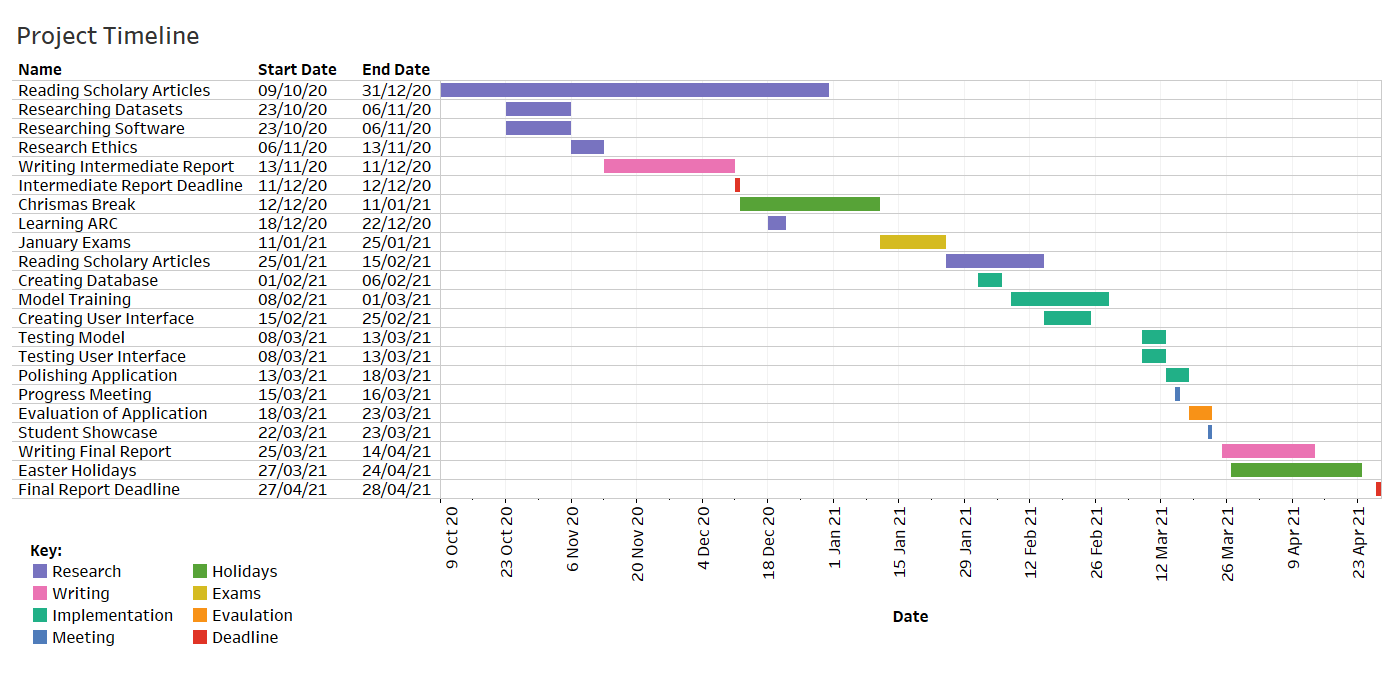
\includegraphics[scale=0.4,center]{intermediateReportTemplateLaTeX/Timeline4.png}
    \caption{A Gantt chart showing the initial plan for the project.}
\end{figure}
After conducting background research, an initial plan was devised. Some time will be allocated to learning ARC, Leeds’ High Performance Graphics cluster over the Christmas period. After, a database will be created using a JetBrains’ DataGrip. Multiple textures will be downloaded from the "Describable Textures Dataset" (DTD) \cite{describingtexturesweb} and the "Flickr Material Database" \cite{materialperceptiondataset}. These textures will be inspected, sorted and then labelled with information about the textures. A table within the database containing references to these images files and their metadata will be created. Additionally, models will be downloaded from Princeton’s ModelNet \cite{volumetricshapesmodeldataset} and standardised so that they are triangulated. Another table will be created in the database with information regarding the files, their UV maps, and metadata for the models. Qt will be used to construct the User Interface and OpenGL will be used to render the 3D models within the User Interface. The pix2pix (source) deep learning framework, implemented in PyTorch, will be used to train and test the model. The this will take place using ARC. Once the model has been train, a User Interface can be created and integrated with the model. 
\subsection{Project Scope}
\label{subsec:projectscope}
One challenging aspect of this project is finding appropriate texture and model resources to use. The UV maps must be accessible beforehand, and a considerable amount of time may have to be spent pre-processing the resources so they are fit to be used on this project. For this reason and the fact that this project is an implementation of Exploratory software, the set of models that can be used by the application will be predefined instead of end-users being able to import their own model files.

\section{Risk mitigation}
\subsection{GAN Model Creation}
\label{subsec:ganmodelcreation}
The GAN model will be trained on Leeds’ High Performance Graphic Clusters (ARC). ARC is a shared system designed for batch processing of high throughput tasks \cite{arcleeds}. Jobs are scheduled between users and are allocated based on availability, number of resources needed and user priority. This means that some time may lie between when the model is ready to train and when the training will actually take place This means that some forethought must be applied concerning how and when to train the model because the system is not readily available. 

\noindent There are several ways to mitigate these problems. It would be best to train the model using the ARC system as few times as possible since the progress of the project is dependant on being allocated a job by the scheduler. Additionally, I have planned to train the model in early February, before starting any development on the UI. This way if any problems with the model are detected, then there is still time to fix them later on in the project. 

\subsection{Illness and Coronavirus}
\label{subsec:illnessandconronavirus}
Due to the Coronavirus epidemic, the last year has been an unprecedented time. The University of Leeds has been impacted in a number of ways by this event. Some services within the University have been slower to respond due to changes in how staff and students have had to adapt to the current climate. This means that some resources may not be as readily available as in the past and response times may be longer than usual. In addition, there is an increased risk of illness within the academic community, that could serve as an obstacle to this project.

\noindent To mitigate this, additional time was added to each task in the initial plan. This means that if something unexpected happens to me or people that I am dependant upon in supporting me in this project, there will still be additional time to spend on this project to make up for it.
\subsection{General Time Management}
\label{subsec:generaltimemanagement}
When devising the initial plan care was taken to ensure that it was a realistic plan and would not conflict with obligations to other modules and exams.
\subsection{Version Control}
\label{subsec:versioncontrol}
There is always the possibility of some unforeseen circumstance (such as a corrupted hard drive or a fire) interfering with this project. For this reason, the version control software 'Git' will be used to manage the source code relating to this project. It will serve as a backup and will also allow for easy accessibility to prior versions. A link to the repository can be found \href{https://github.com/ILeybourne/COMP3931-Individual-Project-Learning-to-Texture-3D-Models}{here}. 